\documentclass{standalone}
\usepackage{tikz} % Import the tikz package
\usetikzlibrary{automata} % Import library for drawing automata
\usetikzlibrary{positioning} % ...positioning nodes
\usetikzlibrary{arrows} % ...customizing arrows
\tikzset{node distance=2.5cm,
    every state/.style={
        semithick,
        fill=gray!10},
    initial text={},
    double distance=2pt,
    every edge/.style={
        draw,
        ->,>=stealth',
        auto,
        semithick}}
\let\epsilon\varepsilon
\begin{document}
    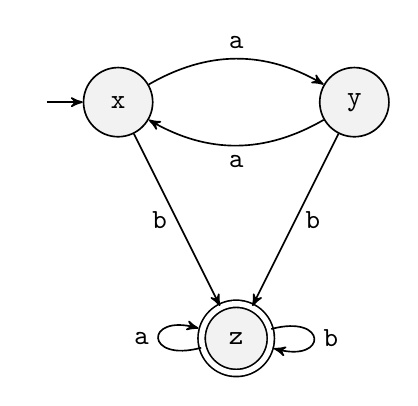
\begin{tikzpicture}
        \node[state,initial] (x) at (0,0) {\tt x};
        \node[state] (y) at (3,0) {\tt y};
        \node[state,accepting] (z) at (1.5,-3) {\tt z};

        \draw (x) edge[bend left] node {\tt a} (y);
        \draw (x) edge[left] node {\tt b} (z);
        
        \draw (y) edge[bend left] node {\tt a} (x);
        \draw (y) edge[right] node {\tt b} (z);

        \draw (z) edge[loop left] node {\tt a} (z);
        \draw (z) edge[loop right] node {\tt b} (z);
    \end{tikzpicture}
\end{document}